\section{Complementarity with Other Experimental Efforts}\label{sec:complementarity}

\subsection{Crossing Symmetry for Thermal Relic Particles}

Production and decay of dark matter particles are often governed by the same or similar interaction. Thermal relic particles such as WIMPs are the textbook example of this situation, where the production through freeze-out from the thermal equilibrium in the early Universe creates the observed relic density~\cite{Srednicki:1988ce, Bertone:2004pz, Feng:2010gw}. The three principal approaches to discover thermal relic particles correspond to the $s$- or $t$-channel processes of dark matter production or scattering, and the time-reversed process to production, which might lead to annihilation of dark matter. This results in the following detection channels, related through crossing symmetry~\cite{Profumo:2013hqa} (see also \autoref{fig:basicfeyn}):

\begin{enumerate}
    \item{\textit{Direct Detection:}} Direct detection of particle dark matter in the Galactic halo in underground experiments as described here;
    \item{\textit{Collider Production:}} Production of dark matter in the laboratory, usually using high energy particle collisions;
    \item{\textit{Indirect Detection}}: Detection of products of dark matter annihilating or decaying in our local universe.
\end{enumerate}

\begin{figure}[!htbp]
\centering
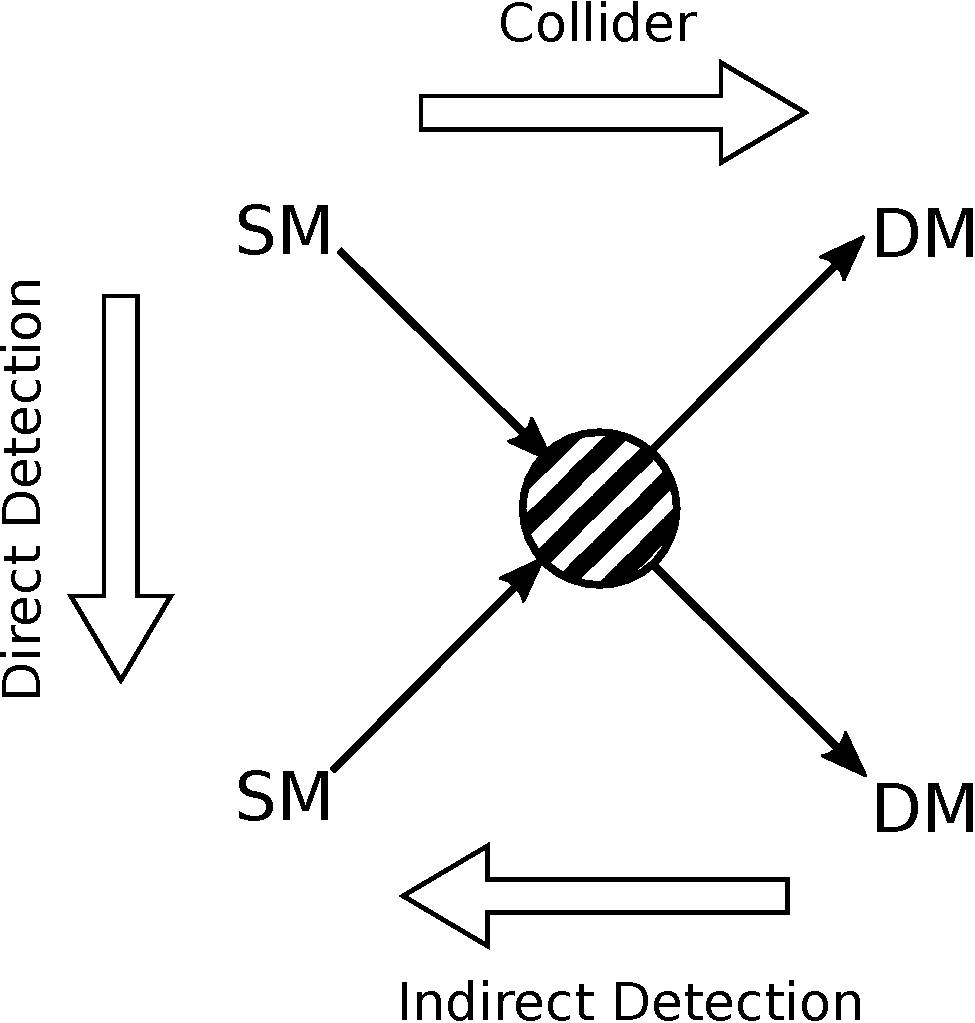
\includegraphics[scale=.3]{fig_basicfeyn.pdf}
\caption{Based on the general idea of thermal relic particles (such as WIMPs) interacting with the standard model, three detection techniques are possible: production at colliders,  scattering from a target material (direct detection) and annihilation resulting in cosmic rays (indirect detection).}
\label{fig:basicfeyn}
\end{figure}

\subsection{Dark Matter at Colliders}

The electroweak energy scale is powerfully probed by the Large Hadron Collider (LHC) at CERN~\cite{Evans:2008zzb}. The freeze-out mechanism requires significant couplings between the dark matter and the standard model, which further motivates searches at a particle collider. Moreover, many `Beyond the Standard Model' (BSM) theories in high energy physics require new particles at the electroweak scale, which are either viable dark matter candidates or might couple to particle dark matter. The most prominent example of such a theory that connects naturally astrophysical and theoretical motivation is supersymmetry (SUSY), which not only remedies many known problems of the Standard Model, such as the hierarchy problem, but also provides an excellent dark matter candidate~\cite{Golfand:1971iw, Clavelli:1970qy, Jungman:1995df, Martin:1997ns}.  

Another motivation for collider searches is the potential to study dark matter in the laboratory. Collider production implies production of the mediator, i.e. the force carrier that connects the dark sector with the visible sector of the Standard Model. Hence, collider dark matter searches are in essence searches for the mediator rather than dark matter. Most collider dark matter searches assume maximal decay of the mediator into dark matter~\cite{Goodman:2010ku, Fox:2011pm}. This is in particular true for 'mono-X' searches, where the main signature is missing momentum in the transverse plane due to the dark matter particle escaping the detector undetected. Constraints placed on the mediator masses are typically about twice as strong as the constraints on the dark matter mass itself. Other analyses attempt to place constraints on the nature of dark matter by looking for deviations in the properties of known particles, for example the Higgs boson, or to search for the mediator directly, such as in dijet searches~\cite{Penning:2017tmb}.

\subsection{Indirect Dark Matter Searches}

Dark matter annihilation and decay into standard model particles lead to potential signatures in the Cosmic Microwave Background~\cite{Finkbeiner:2011dx, Galli:2013dna, Slatyer:2015jla} and astrophysical observables such as X-rays~\cite{Boyarsky:2007ge, Yuksel:2007xh, Perez:2016tcq}, gamma rays~\cite{Gunn:1978gr, Stecker:1978du, Berezinsky:1994wva, Bergstrom:1997fj, Gondolo:1999ef, Gehrels:1999ri, Ullio:2000bv, Cesarini:2003nr, Peirani:2004wy, Dodelson:2007gd, Consortium:2010bc, Cholis:2013ena, Ando:2015qda, Ackermann:2015tah, DiMauro:2015tfa, Ajello:2015mfa, Abdallah:2016ygi, Ahnen:2016qkx, Zitzer:2016fvx, Blanco:2017sbc, Archambault:2017wyh, Lisanti:2017qlb, Ahnen:2017pqx, Abeysekara:2017jxs, Blanco:2018esa, Abdalla:2018mve, Abdallah:2018qtu, Blanco:2019eij}, antiprotons~\cite{Aguilar:2016kjl, Cuoco:2016eej, Cui:2016ppb, Cuoco:2017rxb, Cuoco:2017iax, Cui:2018klo}, positrons~\cite{Cholis:2008hb, Bergstrom:2008gr, Zurek:2008qg, Harnik:2008uu, Cirelli:2008jk, Hooper:2008kg}, neutrinos~\cite{Silk:1985ax, Hagelin:1986gv, Freese:1985qw, Krauss:1985aaa, Gaisser:1986ha, Desai:2004pq, PalomaresRuiz:2007ry, Murase:2012xs, Aartsen:2016zhm, Aartsen:2016fep,  Aartsen:2016pfc, Aartsen:2017ulx}, or other particles~\cite{Ellis:1988qp, Donato:1999gy, Fuke:2005it, Donato:2008yx, Ibarra:2013qt, Hryczuk:2014hpa, Carlson:2014ssa, Aramaki:2015laa, Korsmeier:2017xzj, Reinert:2017aga,Arguelles:2019ouk}. Thermal relic dark matter candidates are generically expected to have a thermally averaged annihilation cross section $\langle\sigma v\rangle \simeq 2.2 \times 10^{-26} \mathrm{cm}^{3} / \mathrm{s}$ ~\cite{Kolb:1990vq, Steigman:2012nb}, though other production mechanisms or annihilation channels are known to predict much smaller or larger annihilation cross sections, e.g., Sommerfeld enhancement~\cite{Hisano:2004ds, ArkaniHamed:2008qn}, non-thermal/out-of-equilibrium production~\cite{Gelmini:2006pq, Gelmini:2006pw, Merle:2013wta, Konig:2016dzg}, asymmetric dark matter~\cite{Graesser:2011wi, Lin:2011gj, Iminniyaz:2011yp, Zurek:2013wia}, co-annihilation~\cite{Griest:1990kh, Edsjo:1997bg, Ellis:1998kh}, velocity-dependent annihilation, or non-standard cosmologies~\cite{Fornengo:2002db, Gelmini:2006pq, Gelmini:2006pw,  Boeckel:2009ej, Boeckel:2011yj, Kane:2015jia, Davoudiasl:2015vba, Berlin:2016gtr, Berlin:2016vnh}. The thermal relic cross section, however, provides an important benchmark for indirect detection efforts. While this leads to a characteristic signature of dark matter in the corresponding cosmic ray spectrum~\cite{Gunn:1978gr, Bergstrom:1997fj, Gaskins:2016cha}, the topology, spectral shape and strength of such a signal is rather model dependent and affected by astrophysical foregrounds.

Since the annihilation rate of dark matter is proportional to the square of the dark matter density at the location of annihilation, the brightest signals are expected to come from dense structures. Present searches for annihilation signatures aim at a variety of targets, with the Galactic center and local spheroidal satellite galaxies (dSphs) of the Milky Way being among the most prominent ones. The former is expected to be the brightest source in the sky because of the large dark matter overdensity, but it also has the brightest foregrounds and complex dynamics. The latter are the most extreme dark matter-dominated galaxies known to us, but have a much lower J-factor~\cite{Abdalla:2016olq, Chiappo:2018mlt} compared to the Galactic center (around $10^{17}-10^{19}\,\rm GeV^2 cm^{-5}$ for dSphs and about $10^{22}\,\rm GeV^2 cm^{-5}$ for the Galactic centre, leading to a fainter potential signal. 

In contrast, the flux of particles from decaying dark matter is only proportional to a single power of density, so it is predicted to give rise to less clumpy signals compared to those from annihilating dark matter. Constraints on decaying dark matter come for example from isotropic gamma-ray and neutrino observations~\cite{Murase:2012xs, Blanco:2018esa}.

There is more than just phenomenological support for the hypothesis that dark matter self-annihilates. $N$-body simulations suggest that dark matter halos, in the absence of baryonic effects, follow a density profile which behaves like $\rho \propto r^{-1}$ irrespective of initial conditions. This is referred to as a Navarro-Frenk-White (NFW) profile~\cite{Navarro:1996gj, Navarro:1996bv}. Measured profiles of dwarf spheroidal galaxies appear to follow a shallower density profile $\rho \propto r^0$. This disagreement is referred to as the `core-cusp-problem' and could possibly be resolved by co-annihilating or self-interacting dark matter (\autoref{sec:selfinteracting}).

\subsection{Measurements of Standard Model Parameters}

In some models of dark matter, the dark matter mass and nucleon-dark matter scattering cross section are predicted or bounded as functions of standard model parameters such as the top quark mass and the strong coupling constant. In such scenarios, dark matter searches constrain the standard model parameters, which can be precisely measured by future colliders~\cite{Seidel:2013sqa,Horiguchi:2013wra,Kiyo:2015ooa,Beneke:2015kwa,Gomez-Ceballos:2013zzn} and lattice QCD computations~\cite{Lepage:2014fla}.

For example, in a model that solves the strong CP problem by a space-time parity symmetry~\cite{Dunsky:2019api}, the dark matter mass is proportional to the energy scale at which the standard model Higgs quartic coupling vanishes ($10^9-10^{12}\1{GeV}$), which is sensitive to the standard model parameters. Dark matter couples to a massless dark photon and the dark matter-nucleon scattering arises from unavoidable quantum corrections leading to photon-dark photon mixing. 

The resultant correlation between the dark matter signal rate and the standard model parameters that determine the scale where the Higgs quartic coupling vanishes is shown in \autoref{fig:mtop_nsig}. Here, to estimate the projections for next-generation experiments, we scale the limit from XENON1T according to the projections in the high mass region shown in \autoref{fig:si_sensitivity}. Another example is sneutrino or higgsino dark matter in supersymmetric theories, where the dark matter mass is predicted to be smaller than the scale at which the standard model Higgs quartic coupling vanishes~\cite{Dunsky:2020yhv}. Dark matter scatters with nuclei via tree-level $Z$~boson exchange, generating signals detectable by $1000t\times y$ exposure even for a dark matter mass as large as $10^{12}$~GeV. Detection of or constraints on nucleon-dark matter scattering signals will give an upper bound on the top quark mass and a lower bound on the strong coupling constant.

\begin{figure}[!htbp]
\centering
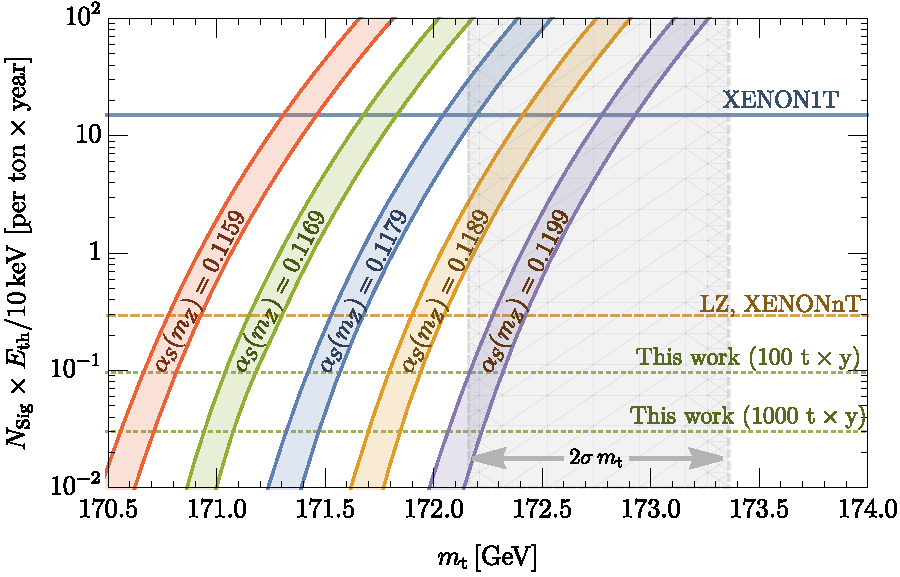
\includegraphics[scale=.52]{fig_mtop_nsig.pdf}
\caption{The expected number of signals per ton$\times$year exposure as a function of the top quark mass, $m_t$, and the strong coupling constant evaluated at the $Z$~boson mass scale, $\alpha_s(m_Z)$, in the model described in~\cite{Dunsky:2019api}. The signal count is inversely proportional to the threshold energy $E_{\rm th}$. The thickness of each colored band corresponds to $2\sigma$ uncertainty in the Higgs mass.}
\label{fig:mtop_nsig}
\end{figure}

\subsection{Other Direct Dark Matter Searches}

In the search for dark matter directly interacting with a laboratory target, a host of synergistic detectors are required to overcome signal degeneracies, particularly as experiments begin probing the neutrino fog. With different technologies and targets, complimentary experiments can confirm potential dark matter signatures and disentangle them from both neutrino-induced (CEvNS) signals and instrumental backgrounds. Additionally, a large variety of detectors can probe a wider dark matter mass range, as shown in \autoref{fig:directdetectionexp}. Target materials range from solid state crystals to dense liquids~\cite{Undagoitia:2015gya, Tanabashi:2018oca}. Even within the context of liquid xenon TPCs, larger detectors are required for dark matter nuclear scattering searches, but smaller detectors optimized for single-electron signals might achieve better sensitivity to lower masses and dark matter scattering with electrons~\cite{Bernstein:2020cpc}. 

\begin{figure}[!htbp]
\centering
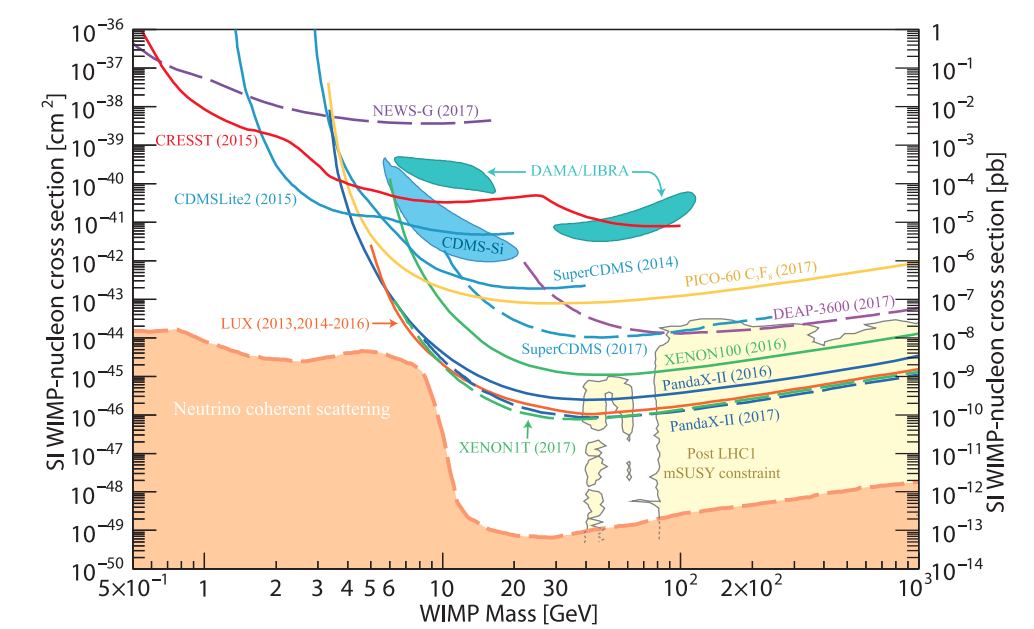
\includegraphics[scale=.24]{fig_directdetectionexp.png}
\caption{Spin-independent dark matter-nuclear scattering limits set by leading direct detection experiments. Complementary experiments with different targets are essential for breaking degeneracies between signals from CEvNS and WIMP dark matter. Additionally, a variety of targets covers a wider range of potential dark matter masses. Figure from~\cite{Tanabashi:2018oca}.}
\label{fig:directdetectionexp}
\end{figure}

\subsubsection{Solid State Detectors}

Germanium detectors (HPGe detectors) are a well-understood target for dark matter searches and have been used particularly by CoGeNT~\cite{Aalseth:2014eft} and EDELWEISS~\cite{Shields:2015wka}. DAMIC~\cite{Aguilar-Arevalo:2016ndq} and SENSEI~\cite{Crisler:2018gci} are using silicon CCDs to look for dark matter interactions, in particular through the electronic recoil channel. SuperCDMS~\cite{Agnese:2014aze} measures both phonons and ionization in silicon and germanium crystals cooled to millikelvin temperatures. CRESST~\cite{CRESST:2019jnq} uses calcium tungstate crystals at millikelvin temperatures to read both phonons and scintillation. Sodium iodide is used by ANAIS~\cite{Amare:2021yyu}, SABRE~\cite{Shields:2015wka} as well as DAMA/LIBRA~\cite{Bernabei:2006tw}. Depending on the target and readout, crystals have different sensitivities to different dark matter interaction energies, but largely overlap across dark matter masses in the GeV and sub-GeV range.

\subsubsection{Liquid Target Detectors}

The PICO experiment~\cite{Amole:2017dex} uses Octafluoropropane in a bubble chamber to search for dark matter-induced signals with a particularly strong sensitivity for spin-dependent interactions. Piezo-electric sensors detect bubble formation in the superheated target during an interaction, and cameras record the bubble nucleation. Perhaps the most complementary experiments to liquid xenon TPCs are liquid argon TPCs, such as DarkSide~\cite{Aalseth:2018gq}. The operating principle is identical to the detector described here, but the smaller atomic mass of argon and its effect on collision kinematics makes Argon invaluable for breaking the energy degeneracy of dark matter scatters and coherent elastic neutrino-nucleus scatters, once observed in liquid xenon TPCs. While self-shielding of external backgrounds is better in xenon, the ability to discriminate electronic from nuclear recoils is better in argon. Taken together, the two target elements provide a complementary approach to probing dark matter down to the signal from atmospheric neutrinos. 

\subsection{Neutrinoless Double Beta Decay Experiments}

Experimental searches for $0\nu\beta\beta$ decay~\cite{DellOro:2016tmg} span a variety of isotopes, including $^{76}$Ge, $^{82}$Se, $^{100}$Mo, $^{130}$Te, $^{136}$Xe, and $^{150}$Nd. The choice of isotope is driven by the Q-value of the $2\nu\beta\beta$ mode, the ability to obtain high isotopic abundance, and compatibility with a suitable detection technique. Detection techniques include semiconductor crystals, cryogenic bolometers, time projection chambers, and organic and inorganic scintillators. The choice of detection technique is a balance of the detector energy resolution at the Q-value, the scalability of the technology to large masses, and ability to achieve ultra low backgrounds. The leading experimental efforts to date include MAJORANA~\cite{Alvis:2019sil}, GERDA~\cite{Agostini:2019hzm}, CUORE~\cite{Adams:2019jhp}, EXO-200~\cite{Anton:2019wmi}, and KamLAND-Zen~\cite{KamLAND-Zen:2016pfg, Gando:2020cxo}. The next generation of $0\nu\beta\beta$ searches includes LEGEND\cite{Abgrall:2017syy}, nEXO~\cite{Albert:2017hjq}, NEXT~\cite{Adams:2020cye}, CUPID~\cite{CUPIDInterestGroup:2019inu}, KamLAND2-Zen~\cite{Nakamura:2020szx}, and SNO+~\cite{Andringa:2015tza}. Compared to the experiments using semiconductors and bolometers, a next-generation liquid xenon detector will have significantly larger isotopic mass, even with a natural abundance of $^{136}$Xe, but it will have poorer energy resolution compared to other technologies. The ability to fiducialize the detector means that the backgrounds from radiogenic sources are significantly reduced. A next-generation liquid xenon dark matter detector can have a $0\nu\beta\beta$ sensitivity comparable to those of the next generation of dedicated $0\nu\beta\beta$ experiments (\autoref{sec:0nubb}). 

\subsection{CEvNS Experiments}

The identification of neutrinos in dark matter experiments, in particular through the CEvNS channel, will be complementary to terrestrial neutrino experiments which operate in a similar energy regime. The COHERENT experiment~\cite{Akimov:2018ghi} uses a stopped-pion source of neutrinos, generated by the Spallation Neutron Source (SNS) at the Oak Ridge National Laboratory. Muon neutrinos with energy $30\1{MeV}$ are produced from charged pion decays, and $\bar{\nu}_\mu$ and $\nu_e$ are produced with a Michel energy spectrum from the subsequent decay of muons at rest. $\bar{\nu}_\mu$ and $\nu_e$ from muon decays are delayed relative to the $30\1{MeV}$ $\nu_\mu$ neutrinos produced from the prompt pion decay. With characteristic energies of tens of MeV, a large sample of the neutrino-nucleus interactions are coherent, which together with the timing structure, permits a measurement of the CEvNS process.

Using 14.6-kg CsI[Na] scintillator detectors, the COHERENT collaboration announced the first detection of CEvNS in 2017~\cite{Akimov:2017ade}, with a best-fit count of 134$\pm$22 CEvNS events, which is 77$\pm$16 percent of the Standard Model prediction. From this initial detection, COHERENT was able to constrain non-standard interactions in a regime of parameter space that had not been possible to probe. In particular, the COHERENT data is sensitive to u- and d-type non-standard interactions for flavor-diagonal muon components, $\epsilon_{\mu \mu}$. The COHERENT detection also set new constraints on exotic solutions to solar neutrino mixing, places novel constraints on new physics that manifests through the neutrino sector (e.g.~\cite{delaVega:2021mhj}), constrains the neutron form factor for CsI~\cite{Ciuffoli:2018qem}, sterile neutrinos~\cite{Coloma:2017egw,Coloma:2017ncl}, and the g-2 anomaly~\cite{Liao:2017uzy}. The collaboration has since also measured CEvNS on Argon~\cite{Akimov:2020pdx}.

Nuclear reactors have been purposed as a copious source of electron anti-neutrinos. The characteristic neutrino energy is $\lesssim 1$ MeV; as such, the coherence condition for the recoil is largely preserved over the entire reactor energy regime. The primary difficulty in detecting CEvNS using reactors is that detectors have not been able to achieve the low threshold required to identify the CEvNS nuclear recoil signal. With new theoretical advances in detector technology, several experiments are poised to identify CEvNS at reactors~\cite{Soma:2014zgm,Aguilar-Arevalo:2016khx,Agnolet:2016zir,Strauss:2017cuu,Leder:2017lva}. The two-phase noble gas detection technique is very promising for this purpose~\cite{Akimov:2019ogx}, and currently the RED-100 detector (with $\sim 160$ kg of active LXe) is being tested at the Kalinin NPP site. It is the first and so far the only one CEvNS experiment using a two-phase emission technique.

\subsection{Solar neutrino experiments}

Direct real-time measurements of solar neutrinos have been observed for the first time by the Borexino experiment~\cite{Arpesella:2007xf, Agostini:2018uly, Agostini:2020mfq}. A next-generation liquid xenon experiments can offer complementary measurements when detecting solar neutrinos through elastic neutrino-electron scattering (\autoref{sec:solarneutrinos}). Neutrinos that contribute to the signal are generated from the $pp$-reaction chain, produced from the electron-capture decay of beryllium-7, and emitted in the carbon, nitrogen, oxygen (CNO) fusion cycle. The measurement of CNO neutrinos in liquid xenon-based detectors is limited by the presence of the two-electron spectrum arising from the $2\nu \beta \beta$-decay of $^{136}$Xe. Depletion of $^{136}$Xe by at least a factor of 100 relative to its natural abundance would be necessary to detect the CNO solar neutrino component in the next-generation xenon-based detector~\cite{Newstead:2018muu}.  

\subsection{Gravitational Wave Searches}

Liquid xenon-based detectors can be utilized to look for neutrinos and gamma-rays released in association with gravitational waves emitted during cataclysmic cosmic events. Such ``simultaneous'' observation is related then to supernova detection and multi-messenger astrophysics, as discussed in \autoref{sec:supernovaneutrinos}.

\subsection{Xenon in Medical Physics}

The two-phase emission detector with condensed xenon working medium has been tested as a high-quality gamma-camera for nuclear medicine \cite{Egorov:1983}. Liquid xenon TPCs have started to come into use for Position Emission Tomography (PET) scans~\cite{Ferrario:2017sgq, GallegoManzano:2015hkg}. In a PET scan, patients are injected with small amounts of chemicals, such as sugar, where molecules have had common stable carbon atoms replaced with positron-emitting isotopes. Position-electron annihilation in the electron shells of atoms in the body leads to back-to-back 511~keV $\gamma$-rays. Cancerous tumors will preferentially absorb more sugar than other parts of the body due to higher rates of metabolic activity~\cite{Kevles:1998}. Liquid xenon is being explored due to its advantageous spatial, temporal, and energy resolutions, combining S1 and S2 information. Many of the developments of this detector technology for particle physics directly benefit these developments.

Compressed xenon gas has been proposed to be used for very effective collimator-less SPECT system or so-called Compton camera~\cite{Bolozdynya:1997ecc, Bolozdynya:1997ccc, Rogers:2004cc}.

Xenon in its gaseous form has also come into use as an alternate anesthetic with minimal dangerous side-effects~\cite{Lynch:2000}. Most oddly and uniquely, there are some studies that suggest it is useful for treating Traumatic Brain Injuries and Post-Traumatic Stress Disorder (PTSD)~\cite{Campos-Pires,Dobrovolsky}. While in the United States these claims have not been evaluated by the Food and Drug Administration (FDA), in Russia, the inhalation of xenon is used for selective ``deletion'' of traumatic memories, associated with negative emotions~\cite{Dobrovolsky}. All this serves to illustrate the extreme versatility of the element. The study of xenon for particle physics may thus have side-effects spilling over into numerous other fields that seem entirely unrelated.

\subsection{Liquid Xenon TPCs for Homeland Security}

The neutron is the gold-standard calibration particle of choice for any WIMP detector, since it is supposed to emulate the nuclear recoil generated by dark matter WIMPs. This implies that a WIMP dark matter detector is also an outstanding neutron detector. Liquid xenon TPCs stationed at seaports and airports can allow for non-intrusive inspection (NII) of fissionable materials in cargo, by detecting gamma rays and fast neutrons emitted spontaneously or by stimulation from nuclear materials~\cite{Nikkel:2012zz}. The ability of discriminating between nuclear and electronic recoils allows to better discriminate against activation from other backgrounds. This holds true even through shielding, given the low $\sim$keV energy thresholds achieved recently for dark matter searches. 

Another homeland security application is monitoring of nuclear reactors at power plants for fuel rod theft, which could change the outgoing neutrino (and not just neutron) flux, or rod type replacement, which could change the balance of uranium and plutonium amounts. This concept has been explored by the Nucifer Experiment~\cite{Boireau:2015dda} with a scintillating liquid. Liquid xenon could be ideal for detecting the resulting change in the rate of CEvNS, already discussed in detail above. Liquid xenon is being considered for detecting CEvNS by the RED collaboration~\cite{Akimov:2019ogx}.

\subsection{Data-Intensive and Computational Sciences}

All of the aforementioned scientific deliverables require the development of cyber-infrastructure such as algorithms, methods, and tools, for the wider benefit of data-intensive sciences. Years of substantial improvements in dark matter detectors means that the field launched into the realm of petabyte data science. The computational science pursued in this field includes, but is not limited to: how ultra-low-energy simulations are performed, including relevant microphysics (\autoref{sec:detector_medium}); how event reconstruction can be performed with the aid of e.g. machine learning~\cite{Khosa:2019qgp}; and how high-throughput/high-level triggers can be deployed on such non-collider experiments.  

This effort requires computational science developments, which can benefit other scientific efforts at both small and large scales. For small scales, there has been an explosion in the number of experiments in recent years. Examples of advancements in this field that are broadly impactful to those having to harness their data are integrating smaller efforts into existing infrastructure using frameworks such as GAUDI~\cite{Barrand:2001ny}; data management systems such as OSG~\cite{Jayatilaka:2017twe}; and demonstrating the effectiveness of columnar compilers in tackling data-intensive applications in high-level descriptive languages. For large scales, overcoming computational science hurdles with novel technologies means serving as a test bed for technologies for Big Science projects such as the HEP Software Project~\cite{Alves:2017she}. Therefore, achieving our physical science goals requires novel computational science and cyber-infrastructure development.


